\todo{Overall I find the motivation section to be disconnected -- you need to
make the connection from incremental VM to frontend analysis, and then to the
need to compile these long-running queries to motivate the confluence.}
\todo{Also make the point that this section surveys the state-of-the-art both
from a research perspective and from an implementation experience perspective.}

In a database system, views are one of the central features in attaining both
logical data independence and efficient performance as evidenced by their use
from query optimization to data integration. While it is clear that improvements
in view maintenance techniques would have a significant impact on a number of
database internals challenges, our form of multilevel views and its realization
as efficient low-level code allows us to provide high-performance, lightweight
monitoring and notification services to the benefit of a wide range of
application domains. Consider the following uses:

\begin{list}{\labelenumi}{\usecounter{enumi} \leftmargin=1em}
\addtolength{\itemsep}{-0.5\baselineskip}
\item An automated stock market trading system monitors the distribution of buy
and sell orders of a particular stock to identify the best time and price for
its own orders.

\item A corporate data warehouse monitors the current status of its production
facilities, warehoused inventory and active demand for its products in order to
preemptively identify supply chain problems.

\item A compute cluster monitors its current status overnight to alert a network
administrator when some of its hardware fails, but only if a distributed task
running on the cluster is at risk of becoming unavailable.
\end{list}

These are all use cases of frontend analysis systems to drive rapid
decision-making and actions in contrast to backend OLAP data warehouses for deep
ad-hoc exploratory querying. These kinds of analysis systems sit on the critical
datapath as close as possible to data sources, inspect events on the fly as part
of alert or automated systems often without human intervention, and are key to
operation or to achieving a competitive advantage. Other examples of application
domains include regulatory compliance~\cite{basel2}, fraud
detection~\cite{ibmfico}, computational
advertising~\cite{agarwal2010forecasting}, steered scientific
simulations~\cite{hey2009fourth} and parameter exploration, disaster
prediction~\cite{scholz1973earthquake}, and online machine
learning~\cite{olesen2008real} amongst others.

Many of the above application domains make heavy use of data management tools,
and while traditional OLTP and OLAP systems are not naturally architected for
dynamic aggregation-heavy analysis queries, it is less clear as to why stream
and complex event, and active database technologies are ill-suited for such
workloads. In addition to discussing the architectural mismatches in stream and
trigger-oriented approaches, we present a preliminary experiment across a range
of query processing engines to demonstrate the update, and view refresh rates
they can attain.

\begin{figure}[htbp]
\begin{tabular}{ p{0.15cm} | l | c | c | c  | c }
\multicolumn{2}{c|}{Query} & \#~Joins    & Where- & Group- & \#~Subqueries\\
\multicolumn{2}{c|}{}      & =: equi     & clause & bys    & and depth\\
                         & & x: cross    &        &        & \\
\hline
\begin{rotate}{90}\hspace{-1.3cm}Finance\end{rotate}
& AXF        & 1, =      & $\vee, <$     & yes & 0 / 0 \\
& BSP        & 1, =      & $\wedge, <$   & yes & 0 / 0 \\
& BSV        & 1, =      & None          & no  & 0 / 0 \\
& MST        & 1, x      & $\wedge, <$   & yes & 2 / 1 \\
& PS         & 1, x      & $\wedge, <$   & no  & 2 / 1 \\
& VWAP       & 0         & $<$           & no  & 2 / 1 \\
\hline
\begin{rotate}{90}\hspace{-1.4cm}TPCH\end{rotate}
& Q3         & 3, =      & $\wedge, <$   & yes & 0 / 0 \\
& Q11        & 2, =      & None          & yes & 0 / 0 \\
& Q17        & 2, =      & $<$           & no  & 1 / 1 \\
& Q18        & 3, =      & $<$           & yes & 1 / 2 \\
& Q22        & 0         & $=,<$         & yes & 2 / 1 \\
& SSB4       & 7, =      & $<$           & yes & 0 / 0 \\
\hline
& SVL        & 0         & $\wedge, <$   & yes & 2 / 1 \\
\end{tabular}
\caption{Features of the algorithmic trading, online decision support, and
cluster monitoring query workload used for experiments.}
\label{fig:queries}
\end{figure}

\vspace{1mm}
\tinysection{Query Workloads for Monitoring}
The above use cases are examples common scenarios in algorithmic trading on
order books, online decision support at a manufacturer, datacenter and network
infrastructure monitoring. 
These update-intensive monitoring applications intrinsically use aggregations
and summarizations, however considering them as flat
select-project-join-aggregate queries is an oversimplification.
In particular, monitoring queries frequently compute a variety of statistics and
compare and contrast them prior to taking action. This leads to queries with
complex dataflows consisting of nested and correlated subqueries composed in
arbitrary fashion amongst other features.
We use a query workload drawn from these domains throughout this paper.
Figure~\ref{fig:queries} lists the salient features of the workload in
terms of processing properties, while their SQL descriptions are listed in
Appendix~\ref{app:queries}.

The algorithmic trading queries operate on two order book tables consisting of
the buy and sell order books present at an electronic stock exchange -- in the
case of our dataset, over a day's worth of orders for the MSFT symbol on NASDAQ
(approx. 2.5 million orders). The online decision support queries are taken from
the TPC-H benchmark, and processed over a update stream replayed in randomized
order from a TPC-H scale factor \todo{0.1} dataset. One additional query in this
scenario is the \todo{SSB4} query that is inspired by the query 4.2 from the
Star Schema Benchmark modified to work on a TPC-H dataset by using one extra
join operation. The cluster monitoring query operates on a synthetic dataset
that simulates tasks running on a 20,000 node cluster.

\todo{More description of query workload, i.e. just verbalize table contents?}

We evaluated this workload on four data management systems, including two stream
processing engines and two popular DBMS, with an open-source (Esper, Postgres)
and commercial implementation (CSPE, CDB)\footnote{We anonymize both of the
commercial systems due to licensing restrictions on publishing benchmarks.} for
each case. We describe implementation specifics below when discussing the
architectural properties of triggers and stream engines. We provide further
details, for example our system specification, with our in-depth experiments in
Section~\ref{sec:experiments}. Figure~\ref{fig:enginecomp} shows the view
maintenance performance achieved by these query processors.
\todo{Check for overlap with experiments section}

\vspace{1mm}
\tinysection{Incremental View Maintenance}
\comment{ In the common approach to incremental view maintenance, a query
optimizer determines delta queries that are then to be evaluated using standard
DBMS physical query plans.}
Despite several decades of research into IVM and its availability in
commercial-grade DBMS\footnote{Postgres does not support materialized views out
of the box, and must be implemented by users as needed.}, there are still many
limitations on its usability. In fact, none of the major DBMS supported
incremental refresh strategies for the majority of our workload when considering
the features listed in Figure~\ref{fig:queries}, and we do not provide a partial
set of experimental results. Inspecting the documentation for many
DBMS~\todo{refs needed here}, the long list of restrictions on supported query
types indicates that view materialization and maintenance cannot be composed in
general fashion with other query optimization and processing concerns. This is a
strong motivator for our research goal of incorporating these aspects as part of
the standard query optimization workflow.
\todo{Give one or two fallacies about IVM.}

\begin{figure}[htbp]
\begin{center}
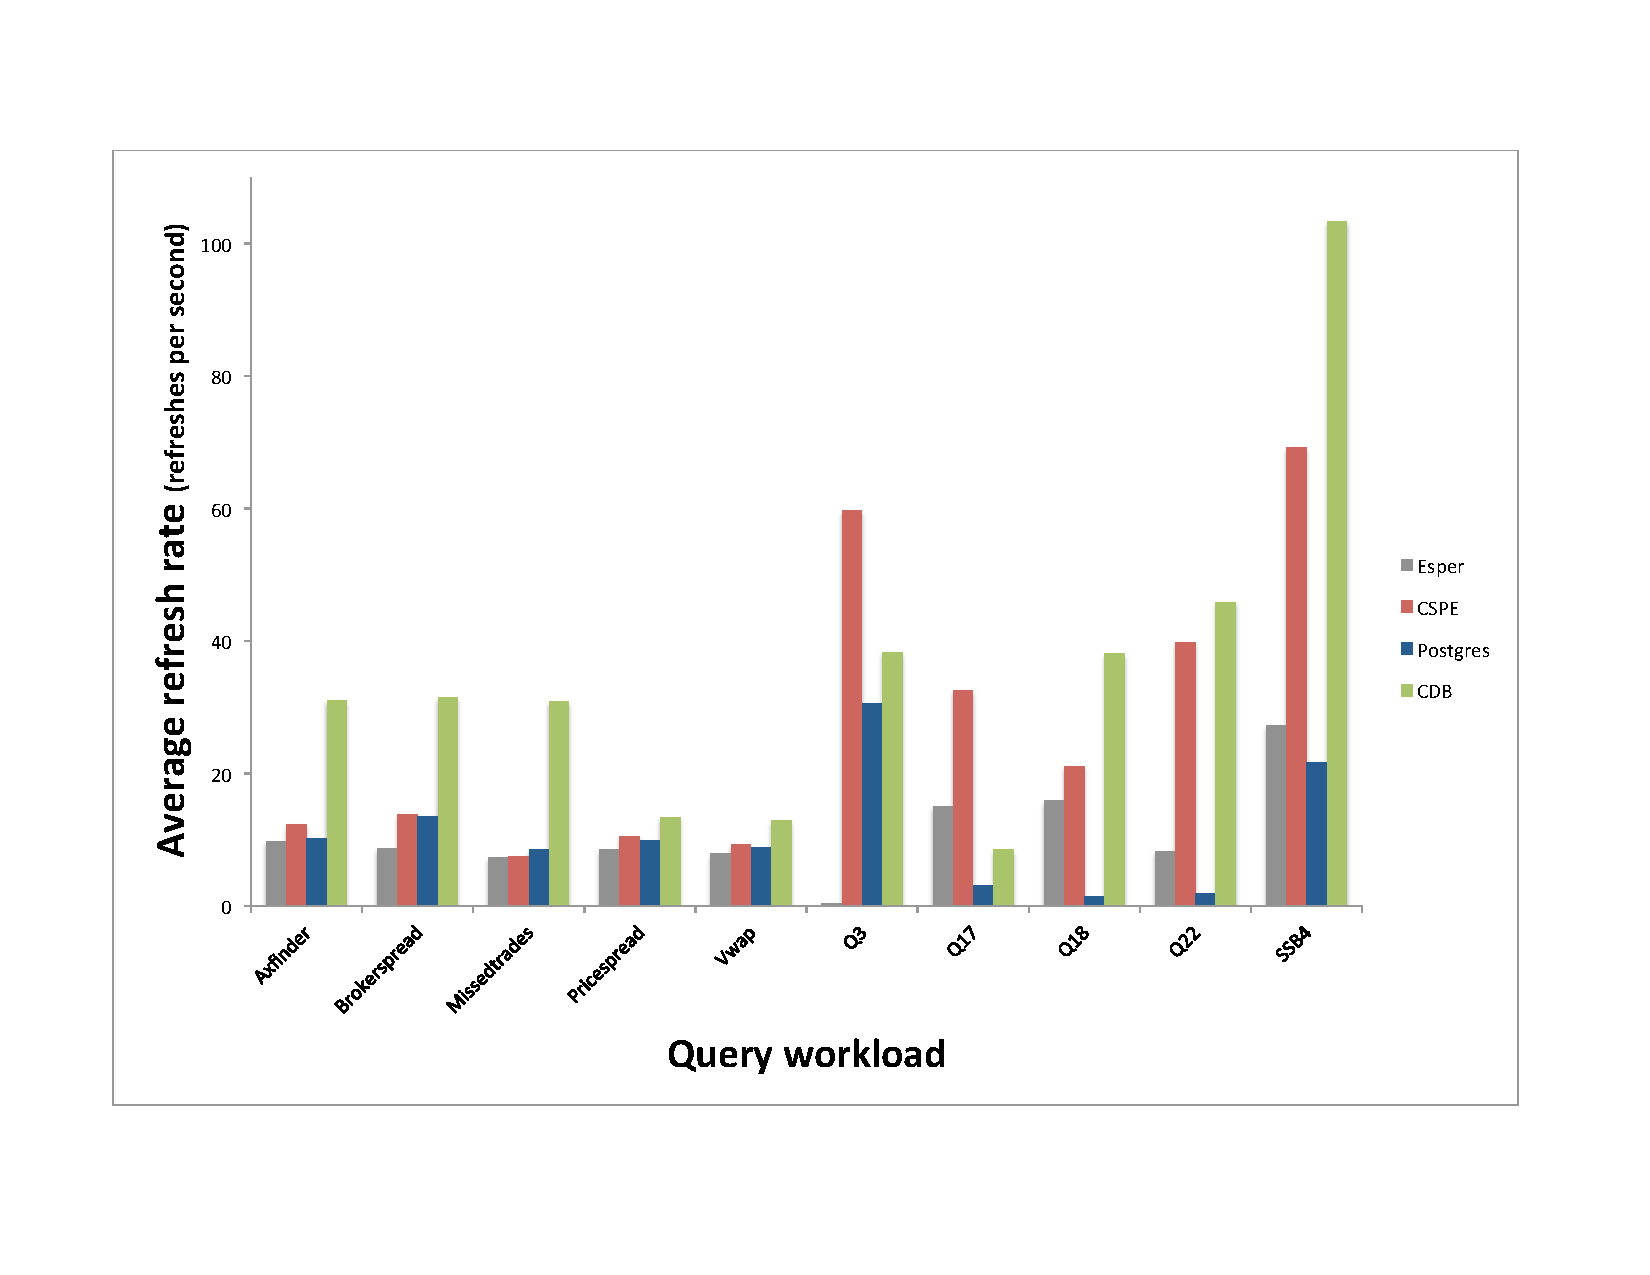
\includegraphics[scale=0.33]{../graphs/graphs/engine-comparison.pdf}
\end{center}
\vspace{-4mm}
\caption{A comparison of four query processing engines implementing full refresh
view maintenance, including both open-source and commercial stream engines and
DBMS.}
\label{fig:enginecomp}
\end{figure}

\vspace{1mm}
\tinysection{Triggers and Active Databases}
Active database methods and their realization as trigger mechanisms in DBMS
allow us to manipulate database state such as indexes and views in a reactive
manner as DML statements execute. Triggers can be implemented in a variety of
procedural and scripting languages from plpgsql, to Python, Java or C. In the
case of procedural SQL languages, triggers undergo the same compilation path as
user-defined queries, that is they are compiled into physical query plans that
are interpreted by the query executor.

Triggers exemplify update processing where the developer looses the ability
for declarative development, and where along with user-defined functions and
aggregates, compilers and query optimizers reside in silos inside a DBMS. Indeed
much of the literature from the database community has focused on issues such as
cascading, recursion and feedback in trigger systems, with limited
work on (single-level) incremental processing that has primarily been drawn from
incremental view maintenance research. Furthermore from an architectural
viewpoint, triggers are built on top of DBMS internals designed for
set-at-a-time computation rather than small granularity, pipelined, and at an
extreme tuple-at-a-time computation.

Using triggers, we implemented a full refresh approach to maintain views for our
query workload. We call this approach \textit{repetitive} processing, where on
each update, a post-update trigger re-evaluates the query from scratch. This
approach incurs minimal developer overhead in performing view maintenance. In
our experience, implementing multilevel view maintenance by hand becomes
impractical very quickly (after even one level of delta transformation) due to
the complexity and number of subqueries that arise, affirming the benefits of
automatic incrementalization during compilation. \todo{Lines of code reference
here.}

\begin{itemize}
  \item Experiment takeaways 
\end{itemize}


\vspace{1mm}
\tinysection{Stream and Complex Event Processing}
Stream and complex event systems (SPEs) provide push-based processing on data
arrival and at first glance may appear to be ideal for frontend analytics. From
an expressiveness standpoint, these systems provide constructs such as windows
or patterns and Kleene closure. Monitoring applications often have additional
requirements -- they must often work with long-lived, large state as essential
application logic, for example an equities order that does not get matched could
potentially reside at the exchange for the entire day or longer, or with
historical data for forecasting. This latter aspect is not well-addressed by the
current generation of stream engines, arising from a disconnect between the
architecture and programmability at the SPE/DBMS boundary that cannot support
incremental computation.

Our workload implementation varied significantly across Esper and CSPE, and in
surveying alternative systems there is a clear lack of standardized semantics
and portability across SPEs. Our implementation strategy involved maintaining
update streams as in-memory tables, replaying relevant tables as updates arrive
to turn tables into streams, and wiring together stream operators to implement
query plans. This essentially constructs fully pipelined physical query
plans and turns out to be very similar to writing trigger code in procedural SQL
languages once the stream is fully replayed.

Additional implementation challenges include computation under looser
transactional semantics. We explicitly restricted our stream implementations to
single-threaded execution and relied on a deterministic tuple processing order
to avoid complexities involving internal scheduling decisions and buffering
present in SPEs. To achieve parallel stream processing, handling these aspects
must make use of locking and barriering strategies (especially with computing
push-based nested aggregates on replayed streams) that added both programming
and performance overheads to our implementation. However our focus in this paper
is primarily on incremental processing as opposed to parallel execution.

\begin{itemize}
  \item Experiment takeaways. blah.
\end{itemize}

